\documentclass{article}

\usepackage[latin1]{inputenc}
\usepackage[T1]{fontenc}
\usepackage[francais]{babel}
\usepackage{graphicx}

\begin{document}

\section{Dimensionnement de l'électroaimant fixe}

Etant donné que nous ne disposons pas d'aimant permanent, nous avons dû fabriquer un électroaimant. 
Nous avons donc bobiné un fil de cuivre autour du matériau ferromagnétique qui nous avait été fourni. 

\begin{figure}[h]
\centering
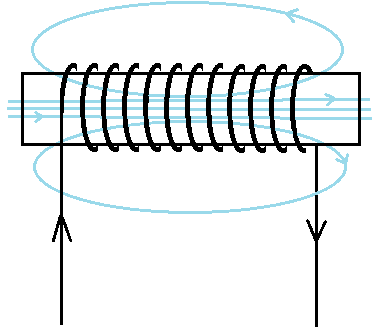
\includegraphics[scale=0.6]{electroaimant.png}
\caption{Modélisation d'un électroaimant}
\label{modélisation de l'électroaimant}
\end{figure}

\paragraph{Fonctionnement}
Lorsqu'un courant traverse la bobine de cuivre, un champ magnétique est formé.  Nous obtenons 
donc un électroaimant fixe générant le champ nécessaire au déplacement de la seconde bobine. 
C'est cette seconde bobine qui sera responsable du tremblement de la membrane.

\begin{figure}[h]
\centering
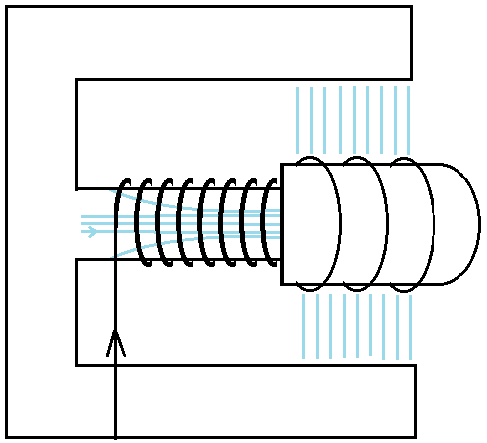
\includegraphics[scale=0.3]{hautparleur.png}
\caption{Vue d'ensemble avec la seconde bobine}
\label{Vue d'ensemble avec la seconde bobine}
\end{figure}

\paragraph{Calul du nombre de spires}
% On doit plutôt dire qu'on fixe le nombre de spires servant à créer le champ
% magnétique à un nombre assez important (Sobieski avait dit 400-500)
% et qu'ensuite on adapte le nombre de spires sur la bobine mobile
% selon les calculs qu'on pourra faire une fois qu'on aura calculer
% la constante de raideur de la membrane.
Dans cete situation, la majorité du champ magnétisant se retrouve dans l'"`entrefer"' de $11$ mm. En supposant qu'il n'y a pas de perte de flux, et que le champ magnétique B vaut  ... T, nous sommes en mesure de calculer le nombre de spires nécessaires pour faire bouger la membrane de $3$ mm. % Peut-être se renseigner sur une valeur typique dans les haut-parleurs
En utilisant les formules suivantes:

$$\oint \vec{H}\cdot\vec{dl}\cong H_m * L + H_e * e = N*I$$ \\
et:
$$B_e = \mu_0*H_e$$\\

Nous obtenons finalement ... spires.

%  ENCORE A DETERMINER

%* nbre de spires
%* éloigné?
%* longueur de la bobine
%* aire du matériau ferromagnétique (combien de plaques)
%* constante de raideur de la membrane

\end{document}